% First Chapter

\chapter{Introduction to Data Quality}

A Web search of terms "data quality" through the search engine Google, returns about three millions of pages
and indicator that data quality issues are real and increasingly important (the term data quality will be shortened to the acronym DQ)

\ifpdf
    \graphicspath{{Chapter1/Figs/Raster/}{Chapter1/Figs/PDF/}{Chapter1/Figs/}}
\else
    \graphicspath{{Chapter1/Figs/Vector/}{Chapter1/Figs/}}
\fi


\section{Why Data Quality is Relevant}

The consequences of poor quality of data are often experienced in everyday life, but often, without making the necessary connections to their causes.

For example, the late or mistaken delivery of a letter is often blamed on a postal service, althought  a closer look often reveals data-related causes, typically an error in the address, orginating in the address database.

Data quality has serious consequences of far-reaching significance, for the efficiency and effectiveness of organizations and business.

\section{Introduction to the Concept of Data Quality}

From a research perspective, data quality has been addressed in different
areas, including statistics, management, and computer science. Statisticians were the first to investigate some of the problems related to data quality, by
proposing a mathematical theory for considering duplicates in statistical data sets, in the late 1960’s. They were followed by researchers in management, who
at the beginning of the 1980’s focused on how to control data manufacturing systems in order to detect and eliminate data quality problems. Only at the
beginning of the 1990's computer scientists begin considering the problem of defining, measuring, and improving the quality of electronic data stored in
databases, data warehouses, and legacy systems.~\citep{CBMS}

Dr. Genichi Taguchi~\citep{Jugulum14}, who was a world-renowned quality engineering expert from Japan, emphasized and established the relationship between
poor quality and overall loss. Dr. Taguchi (1987) used a quality loss func- tion (QLF) to measure the loss associated with quality characteristics
or parameters. The QLF describes the losses that a system suffers from an adjustable characteristic. According to the QLF, the loss increases as
the characteristic y (such as thickness or strength) gets further from the target value (m). In other words, there is a loss associated if the quality
characteristic diverges from the target. Taguchi regards this loss as a loss to society, and somebody must pay for this loss. The results of such losses
include system breakdowns, company failures, company bankruptcies, and so forth.

Figure 1.1 shows how the loss arising from varying (on either side)
from the target by $\Delta_0$ increases and is given by $L(y)$ when $y$ is equal to $m$,

\begin{figure}[htbp!] 
\centering    
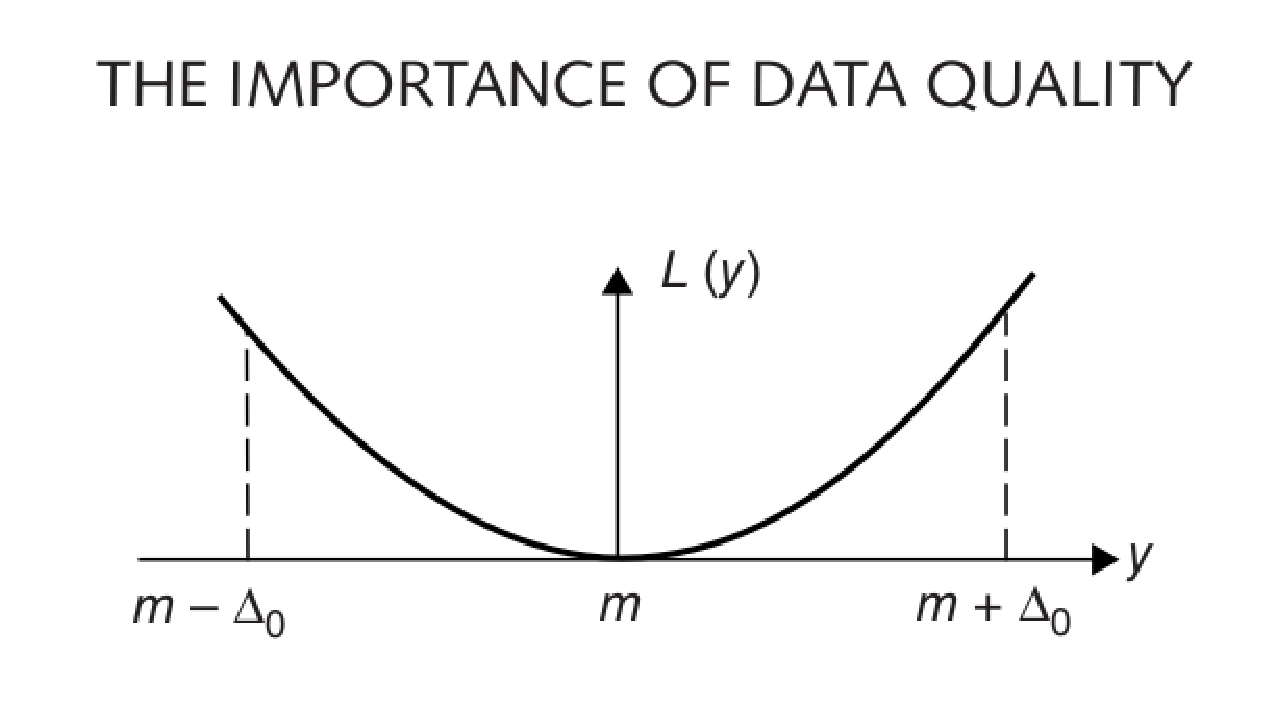
\includegraphics[width=0.6\textwidth]{quality-loss-function}
\caption{Quality Loss Function (QLF)}
\end{figure}

the loss is zero, or at the minimum. The equation for the loss function can
be expressed as follows:

\begin{equation*}
    L(y) = k(y-m)^2
\end{equation*}

where $k$ is a factor that is expressed in dollars, based on direct costs, indi-
rect costs, warranty costs, reputational costs, loss due to lost customers,
and costs associated with rework and rejection. There are prescribed ways
to determine the value of $k$.
The loss function is usually not symmetrical-sometimes it is steep on
one side or on both sides. Deming ~\citep{Deming} says that the loss function need
not be exact and that it is diffi cult to obtain the exact function. As most
cost calculations are based on estimations or predictions, an approximate
function is suffi cient-that is, close approximation is good enough.

The concept of the loss function aptly applies in the DQ context, espe-
cially when we are measuring data quality associated with various data
elements such as customer IDs, social security numbers, and account bal-
ances. Usually, the data elements are prioritized based on certain criteria,
and the quality levels for data elements are measured in terms of percent-
ages (of accuracy, completeness, etc.). The prioritized data elements are
referred to as critical data elements (CDEs).

\section{Data Quality and Types of Information Systems}

Data are collected, stored, elabroted, retrieved, and exchanged in information systems used in organizations to 
provide services to business processes. 
Different criteria can be adopted for classifiying the different types of information systems, and their 
corresponding archirectures; they are usually related to the overall organizational model adopted by the organization or the set of the organizations that make use of the information system.











